\documentclass{article}
\usepackage{graphicx}
\usepackage{hyperref}
\usepackage{multirow}

\begin{document}

\title{Project 4}
\author{Jake Carlson}
\date{November 24, 2017}
\maketitle

\abstract
Clustering

\newpage

\tableofcontents
\newpage

\section{Business Understanding}
This report will focus on clustering analysis of the federal payroll data obtained by BuzzFeed News through the Freedom of Information Act. Specifically, k-means and hierarchical clustering will be used to find groups of emplyees with similar attributes in the federal government.
\par
Armed with an undestanding of what groups exist within each agency, agency leaders can work to create employee teams that are balanced with respect to the features each group holds. We can also see what features create the largest separation between the subgroups.

\section{Data Preparation}
I will prepare my data in a similar fashion to Project 3 \cite{proj3}. I will take the middle of the age range for the age value of each employee. I will do the same thing for length of service. Education will be converted to an integer representing the number of years needed to achieve the degree the employee holds so that all education values are ratio scaled. I will also make supervisory status binary where a one indicates an employee is a supervisor and a zero indicates an employee is not a supervisor. The final list of attributes to be used for clustering is given in Table \ref{tab:1}. Previous projects have shown that Age, Education, Length of Service, Pay, and Supervisory Status are the most relevant employee attributes.
\par
All of these attributes are then scaled. With all of these attributes scaled, I can use Euclidean distance as my distance metric for clustering because all of the attributes are on the same scale.

    \begin{center}
        \begin{table}
            \centering
            \begin{tabular}{ |c|c|c| }
                \hline
                Attribute & Scale & Values \\
                \hline
                Age & Interval & 17, 22, 27, 32, 37, 42, 47, 52, 57, 62, 67, 72, 75 \\
                Education & Ratio & 1 - 22 \\
                LOS & Interval & 1, 3, 7, 12, 17, 22, 27, 32, 35 \\
                Pay & Ratio & 1 - 401,000 \\
                SupervisoryStatus & Nominal & 0, 1 \\
                \hline
            \end{tabular}
            \caption{Final Data Set Attributes}
            \label{tab:1}
        \end{table}
    \end{center}

\section{Modeling}
I will use two clustering methods to compare the structure of the government under Bush and Obama. First I will use k-means clustering. Then I will use hierarchical clusterging.

    \subsection{K-Means}
    K-means attempts to fit the data set by placing k cluster centers and moving them until they cease to move by an amount larger than a given tolerance. It is required that you specify the number of centers to use before the algorithm begins. I will start by first using $k = 3$. I believe this will form groups that represent upper management, middle management, and entry level positions.
    \par
    The location of the cluster centers for the 2005 data set is given in Figure \ref{fig:1}. Here, cluster 2 represents supervisors where the average Pay and Education for the group tends to be higher. The other two clusters represent non-supervisors. Cluster 1 represents employees who are newer and younger, as indicated by the lower Length of Service and Age values. Their Education and Pay is lower than that of cluster 2. Cluster 3 represents employees who are older and have worked for the government for longer, but are not supervisors. Their education is higher than cluster 1, but lower on average than cluster 2. These groupings indicate that employees in the middle age range have a higher likelihood of being supervisors than older employees. Supervisors also tend to have gone to school for longer than non-supervisors.
    \par
    The cluster center locations for the 2013 data set is given in Figure \ref{fig:2}. Again, there is one cluster, cluster 3, that represents the supervisors. Again, the supervisors have an age in the middle of the other two cluster centroids. Cluster 1 represents young employees with some education who are new to working for the federal government. Cluster 2 represents older employees who are not supervisors. This cluster centroid is placed at the lower end of the education axis. I would expect more of the older employees to have a higher level of education, so there is a posibility that the centroid for Cluster 2 is getting stuck in an akward position. To examine this further, I will rerun the clustering for 2013 using $k = 5$ to see if I can get clusters that are more representative of the underlying distribution of employees.
    \par
    The cluster centroids for 2013 with $k = 5$ are given in Figure \ref{fig:3}. We see that the oldest employees have been split by two clusters. In Cluster 4, employees habe a slightly higher education on average and have worked for the government for much longer than employees in Cluster 5. In this clustering, Cluster 3 contains the youngest employees, and Cluster 1 contains employees in the middle of the age range who have the highest levels of education.
    \par
    It still feels like there are more groups hidden in these clusters. To examine how many groups is appropriate for k-means, I will run the algorithm for a varying number of of groups and look at the within sum of squares. By plotting these values and looking for the sharpest turn, we can determine the optimum value for the number of groups to use to cluster this data set using k-means. This plot is given in Figure \ref{fig:4}. The sharpest turn is where $k = 8$, however, the slope increases fairly consistently over the number of clusters, indicating the data can be grouped using any number of clusters and the cluster centroids would still describe relevant features about employees.

    \begin{center}
        \begin{figure}
            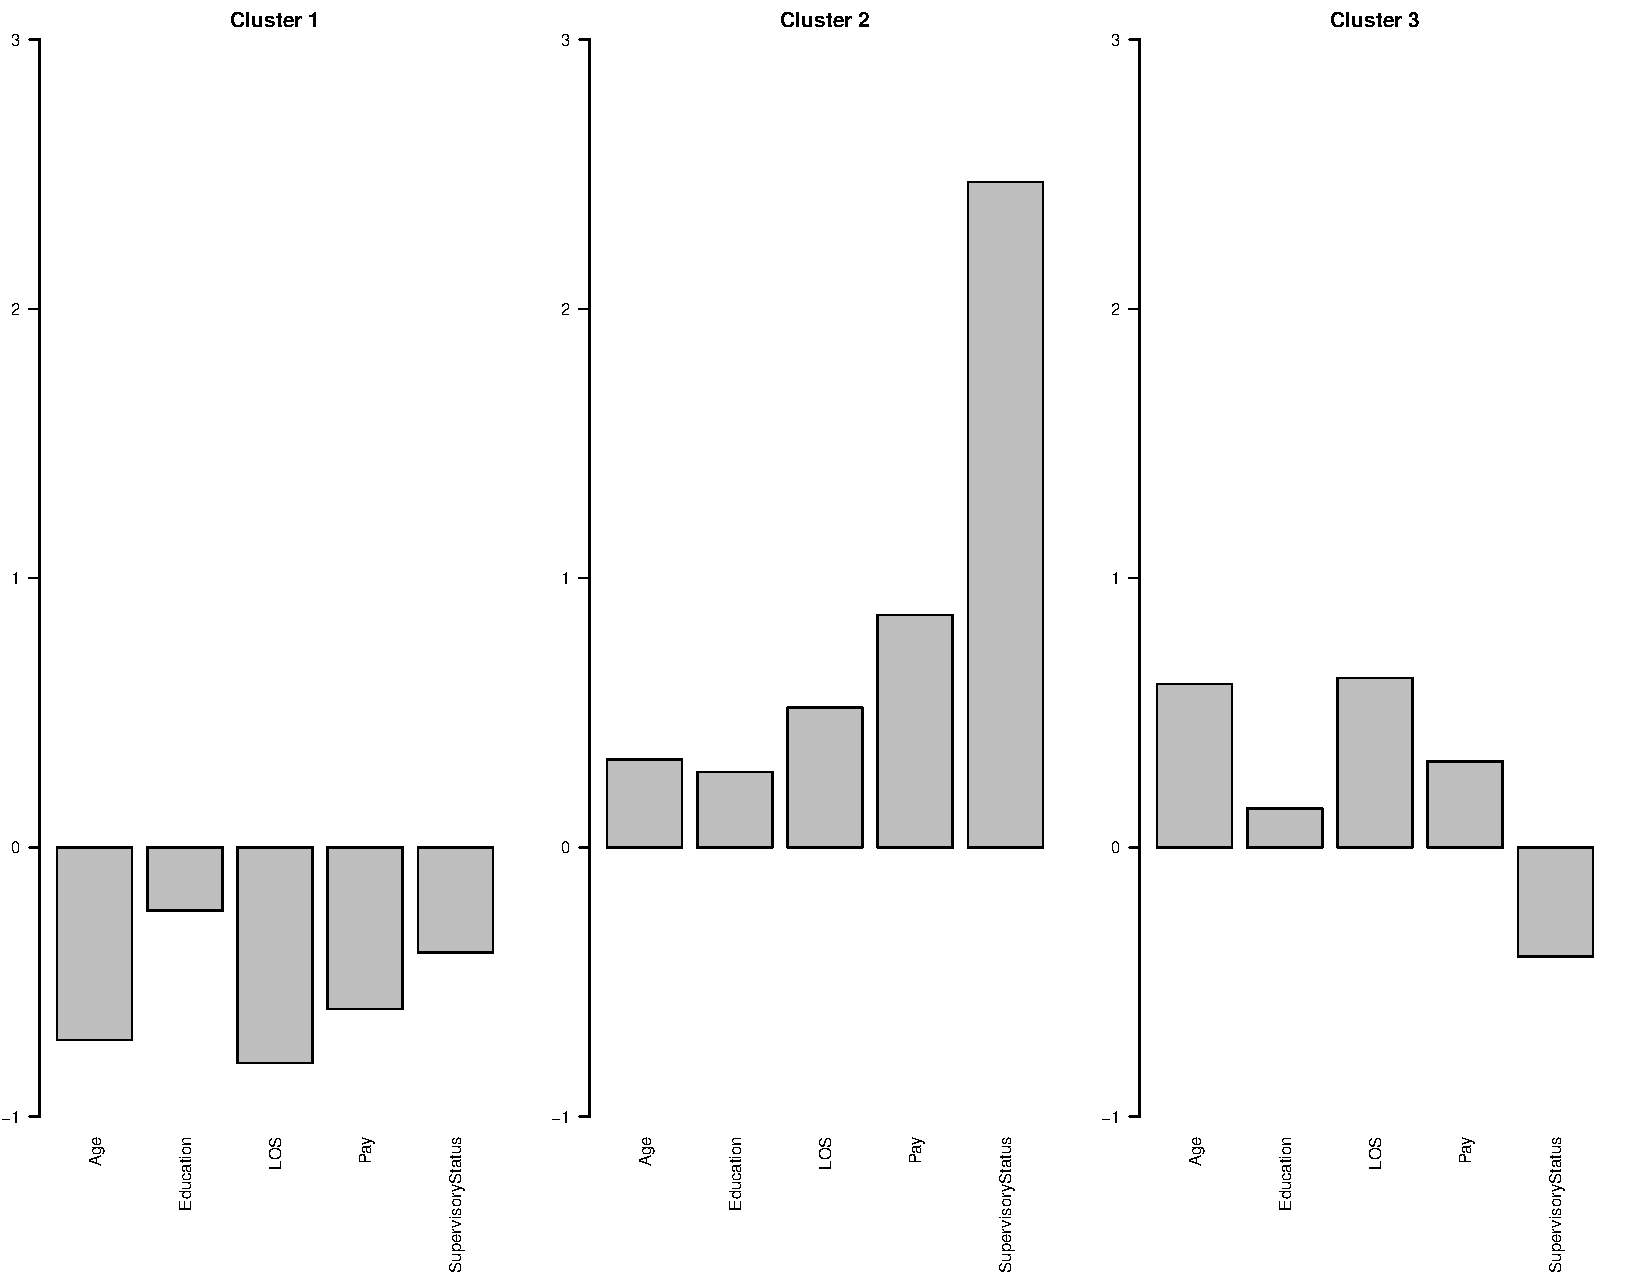
\includegraphics[scale=0.4]{./images/3-cluster-center-2005.pdf}
            \caption{The Location of Cluster Centers for 2005 where k = 3}
            \label{fig:1}
        \end{figure}
    \end{center}

    \begin{center}
        \begin{figure}
            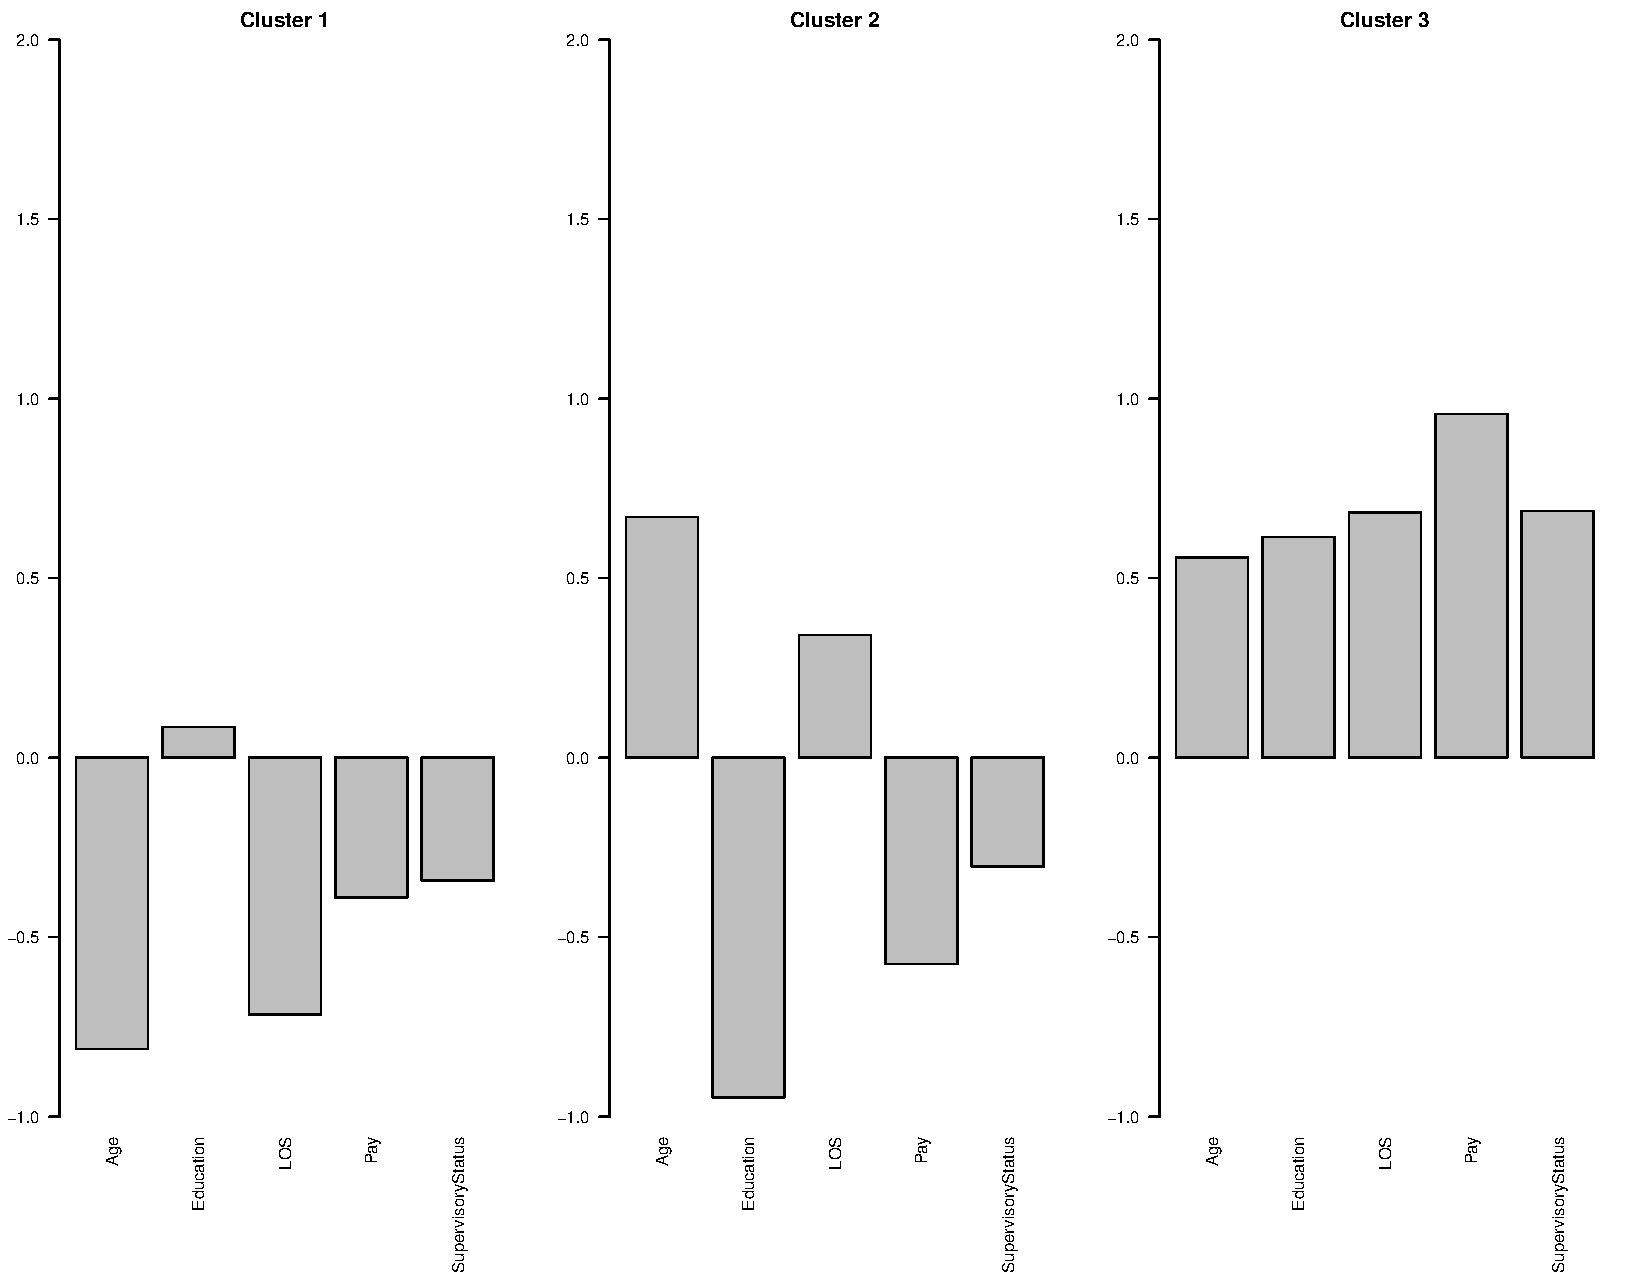
\includegraphics[scale=0.4]{./images/3-cluster-center-2013.pdf}
            \caption{The Location of Cluster Centers for 2013 where k = 3}
            \label{fig:2}
        \end{figure}
    \end{center}

    \begin{center}
        \begin{figure}
            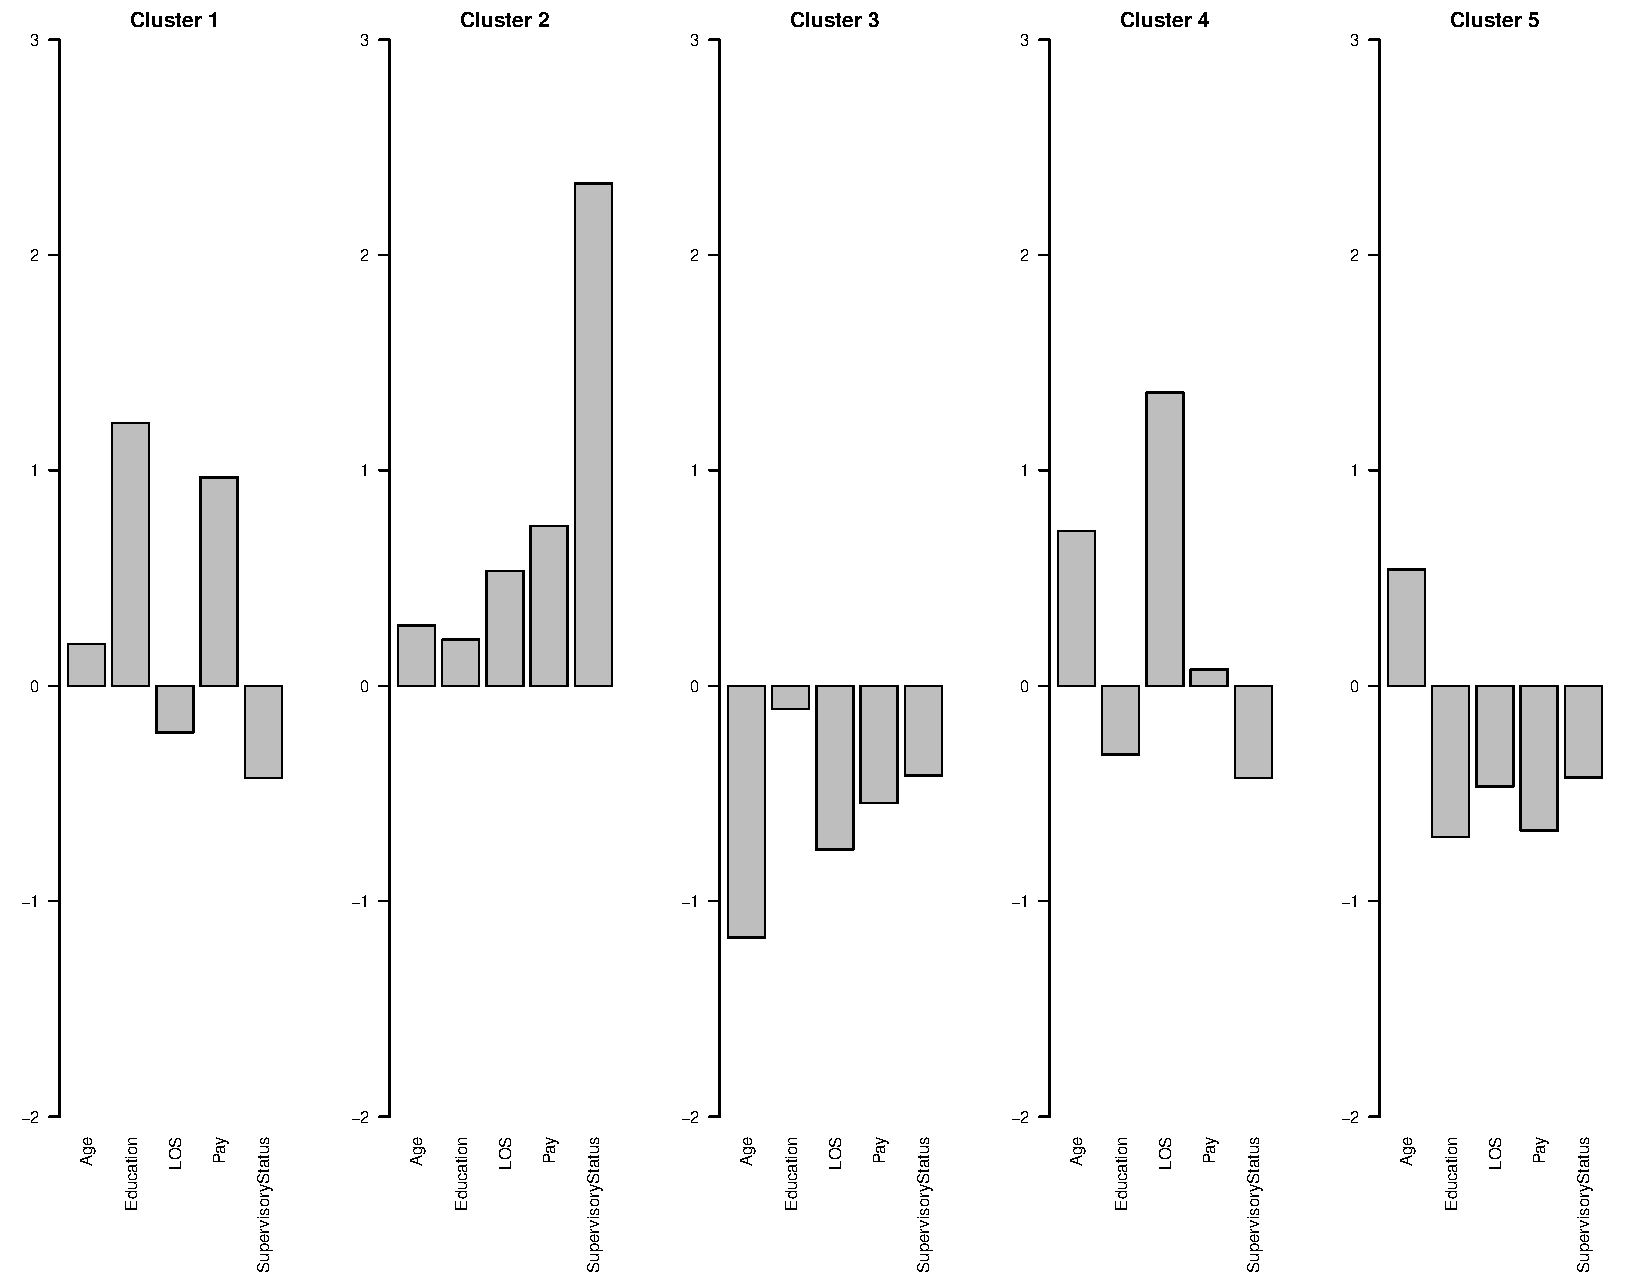
\includegraphics[scale=0.4]{./images/5-cluster-center-2013.pdf}
            \caption{The Location of Cluster Centers for 2013 where k = 5}
            \label{fig:3}
        \end{figure}
    \end{center}

    \begin{center}
        \begin{figure}
            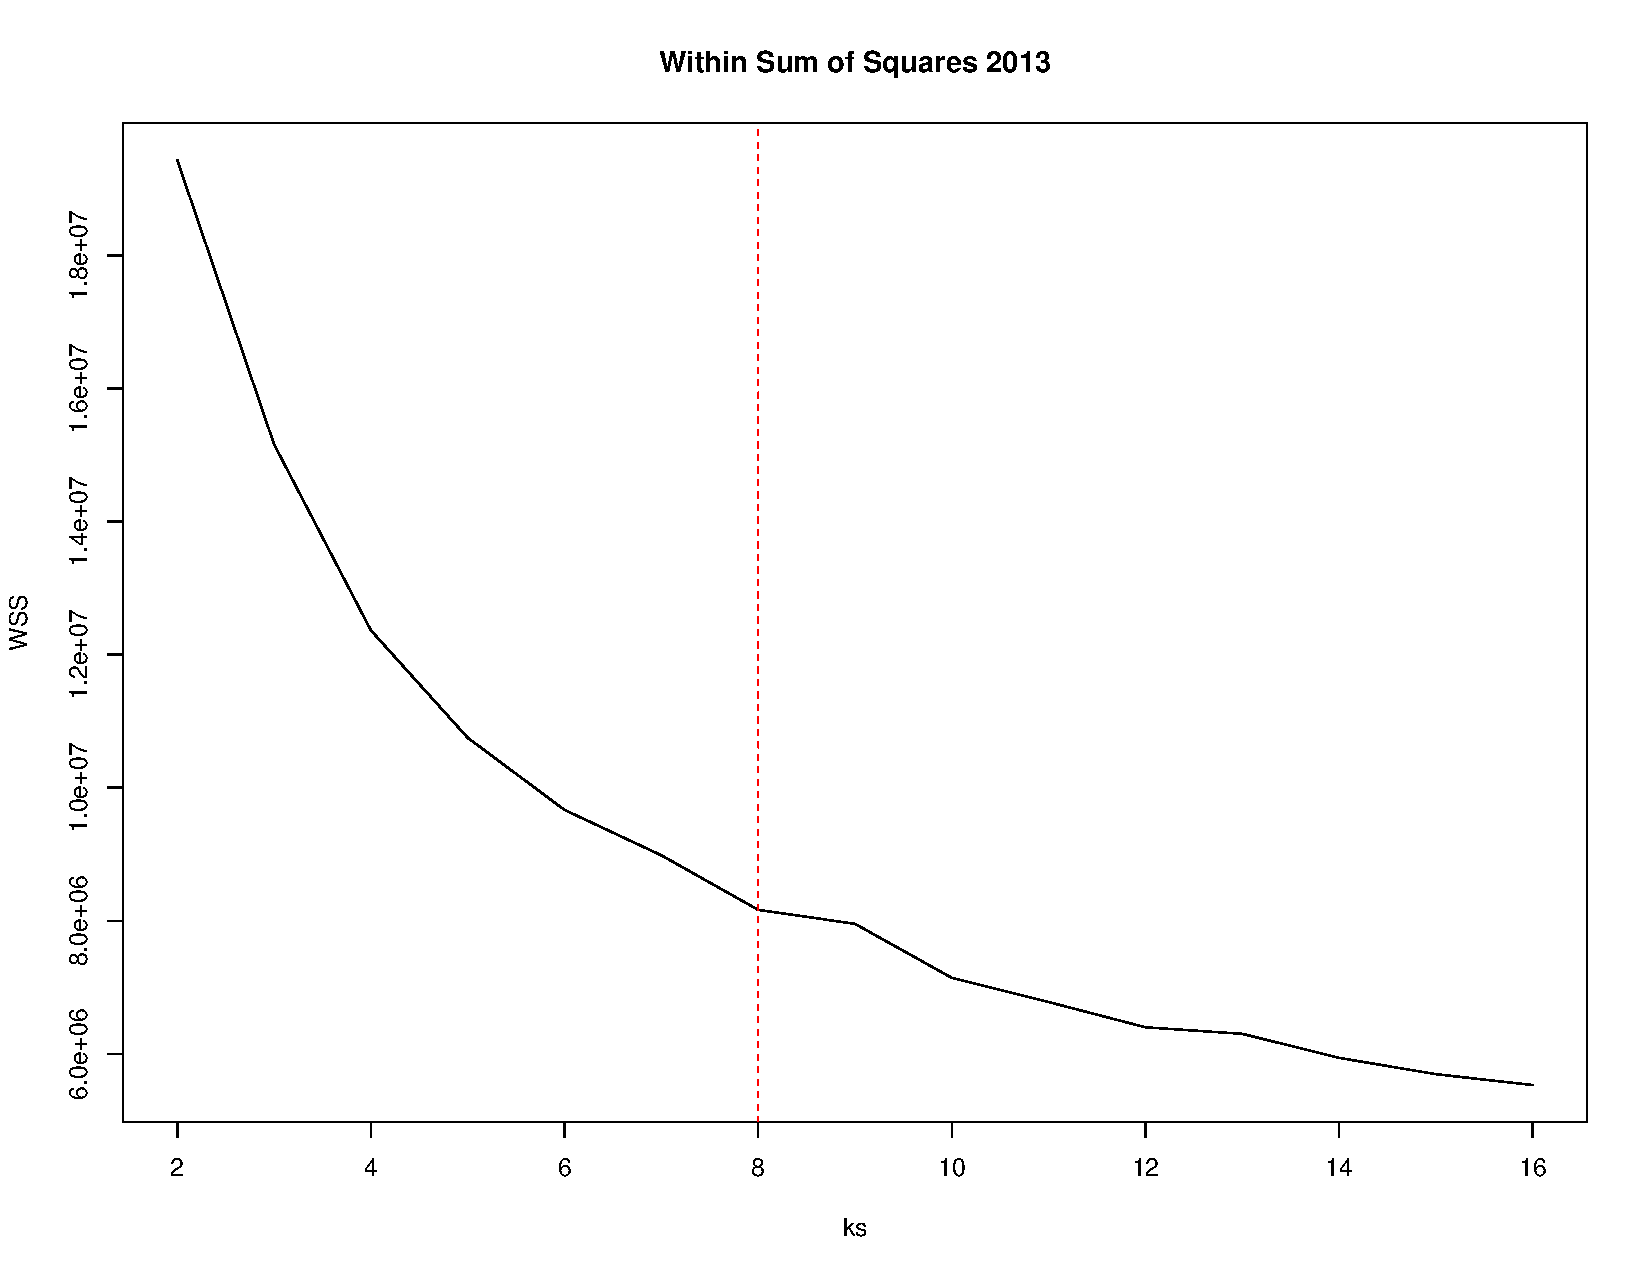
\includegraphics[scale=0.4]{./images/wss-2013.pdf}
            \caption{Within Sum of Squares for 2013}
            \label{fig:3}
        \end{figure}
    \end{center}

    \subsection{Hierarchical}

\section{Evaluation}

\begin{thebibliography}{10}
    \bibitem{proj1}
    Jake Carlson
    \textit{CSE 5331 - Data Mining Project 1}
    \texttt{https://github.com/jakecarlson1/data-mining-projects/blob/master/}
    \texttt{project-1/report/carlson-project-1.pdf}

    \bibitem{proj2}
    Jake Carlson
    \textit{CSE 5331 - Data Mining Project 2}
    \texttt{https://github.com/jakecarlson1/data-mining-projects/blob/master/}
    \texttt{project-2/report/carlson-project-2.pdf}

    \bibitem{proj3}
    Jake Carlson
    \textit{CSE 5331 - Data Mining Project 3}
    \texttt{https://github.com/jakecarlson1/data-mining-projects/blob/master/}
    \texttt{project-3/report/carlson-project-3.pdf}

\end{thebibliography}

\end{document}
